\documentclass{article}
\usepackage[utf8]{inputenc}
\usepackage{amsmath}
\usepackage{graphicx}
\usepackage{tikz}
\usepackage{amssymb}
\usepackage{listings} % for the source code
\usepackage{xcolor} % for the source code as well
\DeclareUnicodeCharacter{2212}{\textendash}

% basic options for putting the source code
\definecolor{codegreen}{rgb}{0,0.6,0} 
\definecolor{codegray}{rgb}{0.5,0.5,0.5} \definecolor{codepurple}{rgb}{0.58,0,0.82} \definecolor{backcolour}{rgb}{0.95,0.95,0.92} 
\lstdefinestyle{mystyle}{ 
    backgroundcolor=\color{backcolour}, 
    commentstyle=\color{codegreen}, 
    keywordstyle=\color{magenta}, 
    numberstyle=\tiny\color{codegray}, 
    stringstyle=\color{codepurple}, 
    basicstyle=\ttfamily\footnotesize, 
    breakatwhitespace=false, 
    breaklines=true, 
    captionpos=b, 
    keepspaces=true, 
    numbers=left, 
    numbersep=5pt, 
    showspaces=false, 
    showstringspaces=false, 
    showtabs=false, 
    tabsize=2 } 
\lstset{style=mystyle}

\title{STAT387 HOMEWORK$\#$2 \linebreak \linebreak
\large INTRODUCTION TO STATISTICAL LEARNING}
\author{Saeah Go}
\date{Due January 29, 12:00 PM}

\begin{document}

\maketitle

\section*{\underline{Conceptual}}
\subsection*{1. 2}
Carefully explain the differences between the KNN classifier and KNN
regression methods. \\
\indent \indent The KNN classifier and KNN regression methods are quite similar. They both are given a value for $K$ and a prediction point $x_0$.
But the difference is that, KNN classifier is usually used to solve \textbf{classification} problems with a qualitative response, by identifying the neighborhood of the study variable $x_0$ and identifying the estimation of the conditional probability, namely $P(Y = j | X = x_0)$ is made, for the class $j$, as a fraction of points in the neighborhood whose response values equals $j$.
But the KNN regression method, is usually used to solve \textbf{regression} problems which are generally associated with a quantitative response by again identifying the neighborhood of $x_0$, and the the $f(x_0)$ is estimated as an average of all the training points of the neighborhood. 


\subsection*{2. 3(a, b)}
Suppose we have a data set with five predictors, $X_1$ = GPA, $X_2$ = IQ,
$X_3$ = Gender ($1$ for Female and $0$ for Male), $X_4$ = Interaction between
GPA and IQ, and $X_5$ = Interaction between GPA and Gender. The
response is starting salary after graduation (in thousands of dollars).
Suppose we use least squares to fit the model, and get $\hat{\beta_0} = 50$, $\hat{\beta_1} = 20$, $\hat{\beta_2} = 0.07$, $\hat{\beta_3} = 35$, $\hat{\beta_4} = 0.01$, $\hat{\beta_5} = −10$. \\
(a) Which answer is correct, and why? \\
\indent i. For a fixed value of IQ and GPA, males earn more on average than females. \\
\indent ii. For a fixed value of IQ and GPA, females earn more on average than males. \\
\indent \textbf{iii. For a fixed value of IQ and GPA, males earn more on average than females provided that the GPA is high enough.} \\
\indent iv. For a fixed value of IQ and GPA, females earn more on average than males provided that the GPA is high enough. \\
\underline{Reason:} \\
The least square line is: 
\begin{center}
$\hat{y} = 50 + 20X_1 + 0.07X_2 + 35X_3 + 0.04X_4 -10X_5$ \\
$= 50 + 20GPA + 0.07IQ + 35Gender$ \\
$+ 0.01GPA\times IQ - 10GPA\times Gender$
\end{center}
If we only observed for males, then, (Note that $0$ is male) 
\begin{center}
$\hat{y} = 50 + 20GPA + 0.07IQ + 35\times 0 + 0.04GPA \times IQ -10GPA \times 0$ \\
$= 50 + 20GPA + 0.07IQ + 0.01GPA\times IQ$
\end{center}
Similarly, for female, (female is $1$)
\begin{center}
$\hat{y} = 50 + 20GPA + 0.07IQ + 35\times 1 + 0.04GPA \times IQ -10GPA \times 1$ \\
$= 85 + 10GPA + 0.07IQ + 0.01GPA\times IQ$
\end{center}
Remember the the response is starting salary after graduation (in thousands of dollars). We can check that the starting salary for males is much higher than for females if $GPA \geq 3.5$. ($\because 50 + 20GPA \geq 85 + 10GPA$) 

\begin{center}
    $50 + 20GPA \geq 85 + 10GPA,$ \\
    $10GPA \geq 35$ \\
    $\therefore GPA \geq 3.5$ \\
\end{center}
Thus the option \textbf{iii} is correct. \\
(b) Predict the salary of a female with IQ of 110 and a GPA of 4.0. \\
For female, the fitted line we get is:  
\begin{center}
    $\hat{y}= 85 + 10GPA + 0.07IQ + 0.01GPA\times IQ$
\end{center}
And we are given that IQ is 110 and GPA is 4.0. We can just put the values.
\begin{center}
    $\hat{y}= 85 + 10\times 4.0 + 0.07\times 110 + 0.01\times 4.0 \times 110$
    $ = 137.1$
\end{center}
Thus we predict the starting salary for the female is: \$137,100 (Since the response is starting salary \underline{in thousand of dollars})

\section*{\underline{Applied}}
\subsection*{3. 8(a, b, c)}
This question involves the use of simple linear regression on the Auto
data set. \\
(a) Use the $lm()$ function to perform a simple linear regression with mpg as the response and horsepower as the predictor. Use the $summary()$ function to print the results. Comment on the output. \\
\indent\indent I used R to answer this question. 
\begin{center}
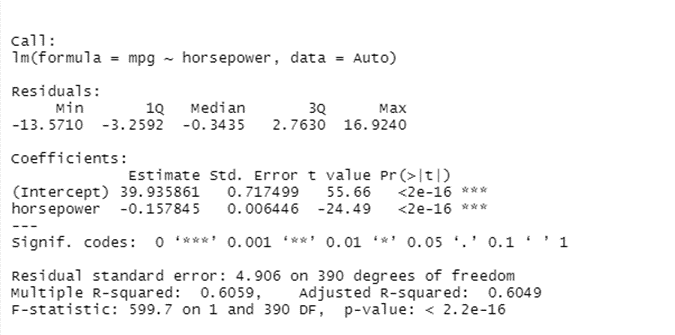
\includegraphics[scale = 0.46]{3.8.a.png} \\
\end{center}
For example: \\
\indent i. Is there a relationship between the predictor and the response? \\
\indent\indent Yes. As we can see in the result above, the p-values for the regression coefficients are nearly zero. ($Pr(>|t|)$ is $<2e-16$) This implies statistical significance, thus we can say that there is a relationship between the predictor and the response. \\
\indent ii. How strong is the relationship between the predictor and the response? \\
\indent\indent The R-squared value is $0.605948$. The $R^2$ value indicates that about $61\%$ of the variation in the response variable ($mpg$) is due to the predictor variable ($horsepower$). \\
\indent iii. Is the relationship between the predictor and the response
positive or negative? \\
\indent\indent Negative. Since the coefficient of the variable `horsepower' is negative ($-0.157845$), the relationship is negative, or specifically we can say inverse relationship exists. \\
\indent iv. What is the predicted mpg associated with a horsepower of
$98$? What are the associated $95\%$ confidence and prediction intervals?
\begin{center}
    $mpg = \beta_0 + \beta_1 horsepower$ \\
    $mpg = 39.94 - 0.16 \times 98$ \\
    \;\;\;\;\;\;\;\;\;\;\;\;\;\; $= 39.94 - 15.68 = 24.26$
\end{center}
Thus, the predicted mpg associated with a horsepower of $98$ is $24.26$ miles per gallon. \\
\linebreak \underline{Confidence Interval \& Prediction Interval} 
\begin{center}
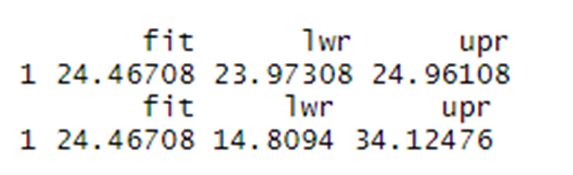
\includegraphics[scale = 0.46]{3.8.a.iv.png} \\
\end{center}
Confidence interval is: [23.97, 24.96] \\
Prediction interval is: [14.81, 34.12] \\
\linebreak (b) Plot the response and the predictor. Use the $abline()$ function
to display the least squares regression line. \\
\indent I used R to answer this question.
\begin{center}
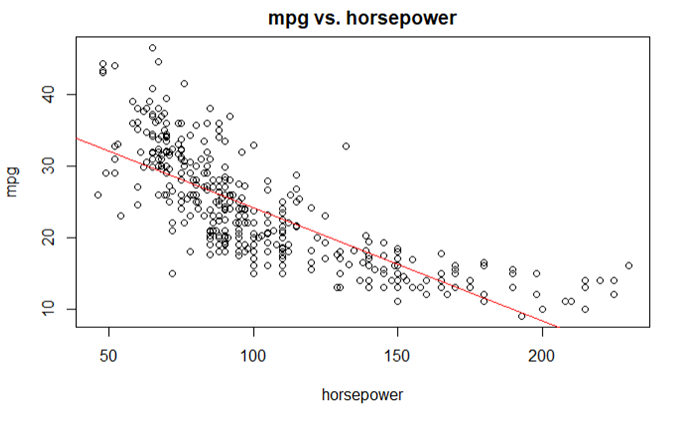
\includegraphics[scale = 0.46]{3.8.b.png} \\
\end{center}
(c) Use the $plot()$ function to produce diagnostic plots of the least squares regression fit. Comment on any problems you see with the fit. \\
\indent I used R to answer this question.
\begin{center}
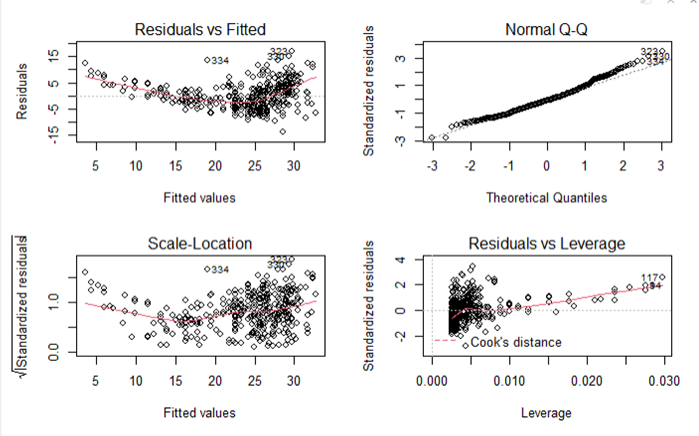
\includegraphics[scale = 0.46]{3.8.c.png} \\
\end{center}
- The first plot (Residuals vs. Fitted) shows a pattern (U-shaped) between the residuals and the fitted values. This indicates a non-linear relationship between the predictor and response variables. \\
- The Normal Q-Q plot (second plot) shows that the residuals are normally distributed. \\
- The third plot (Scale-Location) shows that the variance of the errors is constant. \\
- The fourth plot (Residuals vs. Leverage) indicates that there are no leverage points in the data. % might have some leverage data


\subsection*{4. 10(a, b, c, d, e, f)}
This question should be answered using the Carseats data set. \\
(a) Fit a multiple regression model to predict $Sales$ using $Price$, $Urban$, and $US$. \\
\indent I used R to answer this question.
\begin{center}
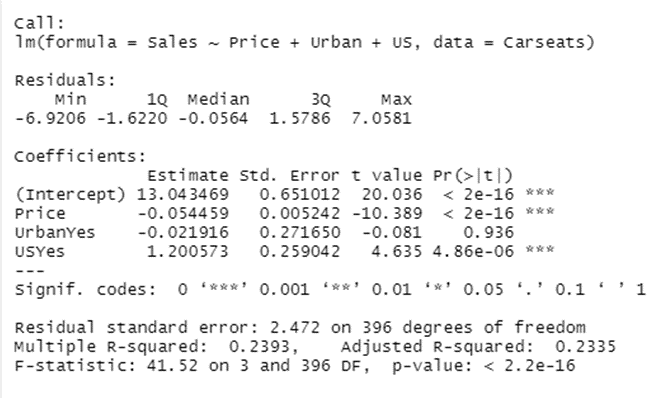
\includegraphics[scale = 0.46]{4.10.a.png} \\
\end{center}
(b) Provide an interpretation of each coefficient in the model. Be careful - some of the variables in the model are qualitative! \\
\indent \indent The coefficient of Price is $-0.054459$. Note that Sales is unit sales (in thousands) at each location. So, when price increases by $\$1000$ and other predictors are held constant, sales decrease by $54.459$ unit sales. In other words, when price increases by $\$1000$, the number of car-seats sold decrease by $54.459$. \\
\indent \indent Note that the predictors Urban and US are qualitative. A store’s sale is not much affected much by whether the store is in Urban area or not. We could notice this since the p-value of Urban is really high ($0.936   > 0.05$ which means the predictor Urban is not significant) and the coefficient is close to zero ($-0.021916$). But we can still say that a store's sale is approximately $22$ less car-seats than a store in rural area. \\
Since the coefficient of the predictor US is $1.200573$, store in the US sales $1201$ more car-seats (in average) than a store that is abroad. \\
\linebreak (c) Write out the model in equation form, being careful to handle the qualitative variables properly. \\
\indent I rounded to the nearest thousandth.
\begin{center}
    $Sales = 13.043 - 0.054Price - 0.022Urban + 1.201US$ % + \epsilon$
\end{center}
\indent \indent Or we can rewrite this for each situation.
\begin{center}
    $Sales = 13.0435 − 0.054Price − 0.022 + 1.201$ (if store is in urban US area) \\ 
    $Sales = 13.0435 − 0.054Price + 1.201$ (if store is in the rural US area) \\
    $Sales = 13.0435 − 0.054Price − 0.0219$ (if store is non-US urban area) \\
    $Sales = 13.0435 − 0.054Price$ (if store is not in the US and not in urban area)
\end{center}
(d) For which of the predictors can you reject the null hypothesis $H_0$ : $\beta_j = 0$? \\
\indent \indent We reject the null hypothesis when p-value is less than $0.05$. In this case, we can check that the p-value of the predictor Price is $< 2e-16$ and the p-value of the predictor US is $4.86e-06$. Thus the predictors Price and US, we can reject the null hypothesis $H_0$ : $\beta_j = 0$. \\
\linebreak (e) On the basis of your response to the previous question, fit a smaller model that only uses the predictors for which there is evidence of association with the outcome. \\
\indent I used R to answer this question.
\begin{center}
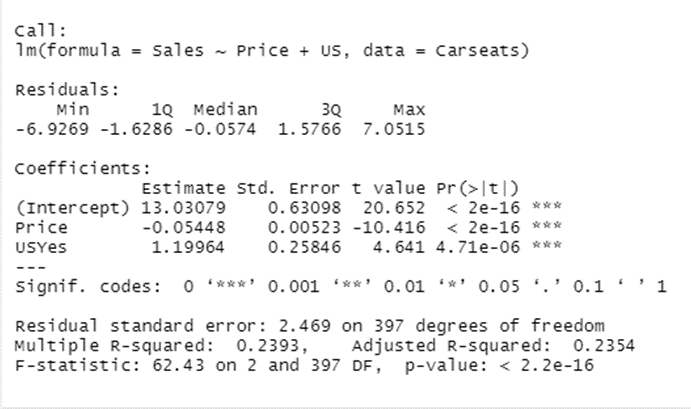
\includegraphics[scale = 0.46]{4.10.e.png} \\
\end{center}
(f) How well do the models in $(a)$ and $(e)$ fit the data? \\
\indent The smaller (reduced) model that we made in $(e)$ is a bit better, since the adjusted $R^2$ value is slightly higher. The adjusted R-squared for $(a)$ is $0.2335$ and the adjusted R-squared value for $(e)$ is $0.2354$.

\subsection*{5. 13(a, b, c, d, e)}
In this exercise you will create some simulated data and will fit simple
linear regression models to it. Make sure to use set.seed(1) prior to
starting part (a) to ensure consistent results. \\
(a) Using the $rnorm()$ function, create a vector, $x$, containing $100$
observations drawn from a $N(0, 1)$ distribution. This represents a feature, $X$. \\
\indent I used R to answer this question. \\
\linebreak (b) Using the $rnorm()$ function, create a vector, $eps$, containing $100$ observations drawn from a $N(0, 0.25)$ distribution $i.e.$ a normal
distribution with mean zero and variance $0.25$. \\
\indent I used R to answer this question. \\
\linebreak (c) Using $x$ and $eps$, generate a vector $y$ according to the model \\
\begin{center}
$Y = −1+0.5X + \epsilon$ 
\end{center}
What is the length of the vector $y$? What are the values of $\beta_0$
and $\beta_1$ in this linear model? \\
\indent I used R to answer this question. \\
\indent The length of the vector $y$ is $100$. The values of $\beta_0$ is $-1$ and $\beta_1$ is $0.5$. \\
\linebreak (d) Create a scatter plot displaying the relationship between $x$ and
$y$. Comment on what you observe. \\
\indent I used R to answer this question.
\begin{center}
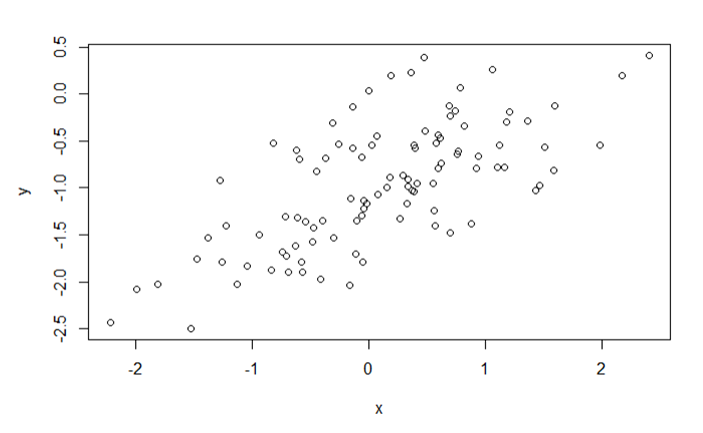
\includegraphics[scale = 0.46]{5.13.d.png} \\
\end{center}
\indent \indent The data points are moderately spread out, but the values of $y$ increases as we move right along the $x$ axis. Thus we can conclude that between the variables $x$ and $y$, the relationship is quite positive. \\
\linebreak (e) Fit a least squares linear model to predict $y$ using $x$. Comment on the model obtained. How do $\hat{\beta_0}$ and $\hat{\beta_1}$ compare to $\beta_0$ and $\beta_1$? \\
\indent I used R to answer this question.
\begin{center}
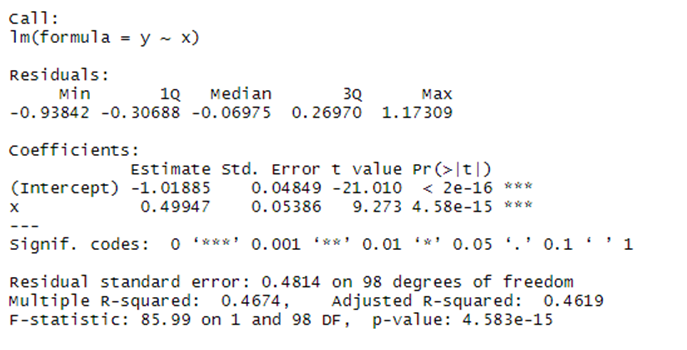
\includegraphics[scale = 0.46]{5.13.e.png} \\
\end{center}
\indent \indent Based on the result above, the estimated regression line is: 
\begin{center}
    $\hat{y} = -1.01885 + 0.49947x$
\end{center} 
\indent \indent The $R^2$ value is 0.4674, and this indicates that 46.94\% variation in $y$ is explained by the model. The predictor $x$ is significant because the p-value is $4.583e-15$. The positive coefficient 0.4995 (slope) indicates that $x$ and $y$ have a positive relationship. In other words, it means that for one unit increase in $x$, $y$ increases by 0.4995. \\
\indent We can check that the estimated values of the coefficients ($\hat{\beta_0}, \hat{\beta_1}$) are pretty close to the true values ($\beta_0, \beta_1$).
$\hat{\beta_0} = -1.0188, \hat{\beta_1} = 0.4995$ \\
$\beta_0 = -1, \beta_1 = 0.5$

\section*{\underline{R Code}}
\begin{lstlisting}[language=R]
# Applied

#################################
## 3.8 (a, b, c)
#################################
### Problem (a)
data(Auto) # load the data
fix(Auto) 
fit1 <- lm(mpg ~ horsepower, data = Auto)
summary(fit1)

# get the associated 95 % confidence interval
predict(fit1, data.frame(horsepower = 98), interval = "confidence")

# get the associated 95 % prediction interval
predict(fit1, data.frame(horsepower = 98), interval = "prediction")


### Problem (b)
plot(Auto$horsepower, Auto$mpg,
     main = "mpg vs. horsepower",
     xlab = "horsepower",
     ylab = "mpg")
abline(fit1,
       col = "red") # make the line color to red to easily see


### Problem (c)
par(mfrow = c(2, 2)) # two columns two rows
plot(fit1)






#################################
## 4. 10 (a, b, c, d, e, f)
#################################
### Problem (a)
data(Carseats)
fix(Carseats)

fit2 <- lm(Sales ~ Price + Urban + US, data = Carseats)
summary(fit2)


### Problem (e)
fit3 <- lm(Sales ~ Price + US, data = Carseats)
summary(fit3)






#################################
## 5. 13(a, b, c, d, e)
#################################
### Problem (a)
set.seed(1)
x = rnorm(100)


### Problem (b)
eps = rnorm(100, sd = sqrt(0.25)) # variance = sd^2 # eps is epsilon (error term)


### Problem (c)
y = -1 + 0.5 * X + eps
length(y)


### Problem (d)
plot(x, y)


### Problem (e)
fit4 <- lm(y ~ x)
summary(fit4)
\end{lstlisting}
\end{document}